Discourse, in English, denotes written and spoken communications. Formally, it is a conceptual generalization of conversation within each modality and context of communication.  Because a discourse is a body of text meant to communicate information and knowledge, there exists a variety of types of relations in the content of a discourse, which composes the internal structure of the discourse. For example, rhetorical relations explain coherence by postulating a hierarchical connected structure of texts (shown in figure \ref{fig:dis_intro}). We see that a single text span ``it does have beautiful scenery'' is elaborated and supported by its context ``some of the best since Lord of the Rings''. Study on uncovering latent structures of discourse is called discourse analysis in natural language processing (NLP). It's main idea is to understand how context affects the meaning of the sentence. This contrasts with a group of NLP studies based on smaller bits of language, such as sounds (phonetics and phonology), parts of words (morphology), and meaning (semantics).  %For example, Charles Fillmore points out that two sentences taken together as a single discourse can have meanings different from each one taken separately. To illustrate, he asks you to imagine two independent signs at a swimming pool: "Please use the toilet, not the pool," says one. The other announces, "Pool for members only." If you regard each sign independently, they seem quite reasonable. But taking them together as a single discourse makes you go back and revise your interpretation of the first sentence after you've read the second.

%we show the discourse structure of a movie review indicated by  Rhetorical Structure Theory (RST).
 
We study the connection between discourse structure and text based applications. Previous work has shown a great success on modeling discourse structure as latent features to solve downstream NLP tasks. Ji \cite{ji2016latent2} presents a latent variable recurrent neural network architecture for jointly building a language model and understanding latent discourse relations. Li \cite{li2018joint} shows that the jointly modeled discourse and topic representations can effectively indicate summary-worthy content in microblog conversations. Nejat \cite{nejat2017exploring} provides evidences that information extracted from Discourse Trees can help with Sentiment Analysis and likewise, knowing the sentiment of two pieces of text can help with identification of discourse relationships between them.  

We focus on two particular types of discourse, speech act\footnote{In many scenarios, speech act and dialogue act both mean the same thing. We will use them interchangeably in the following sections.} and discourse marker:

\begin{enumerate}
    \item \textbf{Speech Act} is an utterance expressed by an individual that not only presents information, but performs an action as well. %Saying "I now pronounce you man and wife" enacts a marriage. 
    Speech acts serve their function once they are said or communicated. These are commonly taken to include acts such as apologizing, promising, ordering, answering, requesting, complaining, warning, inviting, refusing, and congratulating. Studying the speech act in discourse can help us discover the discourse structure. In figure \ref{fig:dis_intro}, the utterance ``It would be comfortable to hold on also.'' said by speaker E is labeled with \texttt{Elaboration}, and connected to the previous utterance, so \texttt{Elaboration} can be seen as the discourse relation between these two utterances. This utterance is considered as a speech act as it expresses the speaker's idea ``rubber is more comfortable'', as well as presenting an agreement on speaker A's proposal.
    
    \item \textbf{Discourse Marker} is the term linguists give to common words like ``well'', ``oh'', ``but'', ``and'' etc, that break text up into integral segments and show the relation between them. For example, ``Oh'' prepares the hearer for a surprising or just-remembered item, and ``but'' indicates that the sentence to follow is in opposition to the one before. However, these markers don't necessarily mean what the dictionary says they mean. Some people use ``and'' just to start a new thought, while others put ``but'' at the end of their sentences, as a way of trailing off gently. We can see that these discourse markers work as explicit discourse structure cues. It is simple to identify the discourse relation between two utterance if it is signaled by a discourse marker. %Realizing that these words can function as discourse markers is important to prevent the frustration that can be experienced if you expect every word to have its dictionary meaning every time it's used.
\end{enumerate}

\begin{figure}[t] 
\centering
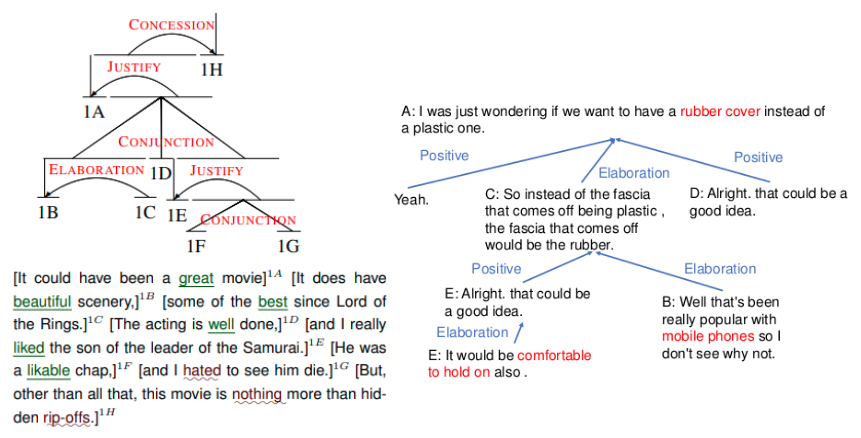
\includegraphics[width=1.0\columnwidth]{Images/dis_intro.png} 
  \caption{\textbf{Left side:} an example of RST discourse structure. We show the rhetorical relations between text spans in red. \textbf{Right side:} A meeting snippet. A, B, C, and E denotes different speakers. We show the attachment structure and the type of the speech act in blue.}
\end{figure}\label{fig:dis_intro} 

In this chapter, we study discourse in both spoken contexts and written texts, modeling discourse structures as latent variables. To fit into a machine learning framework, we will figure out ways to represent them as real value discrete random variables. Then we investigate the best model structure that can help us link the latent variable to the learning target, and estimate the value of the latent variable. We propose to use log-linear model, reinforcement learning, and sampling-based inference as our base models and learning methods. As we discussed earlier in section \ref{sec:ch-1}, latent information can be used to evaluate the performance of the model and improve the interpretability of the learning process. We will demonstrate several ways to interpret prediction process by using latent information. Furthermore, we will show learned latent discourse structure can help us solve downstream tasks. Because discourse is not observable, we cannot feed it as numerical features to classifiers directly. We will rely on inference step of our model to build features based on its outputs.

In section \ref{sec:3-1}, we will first present a joint modeling approach to identify salient discussion points in spoken meetings as well as to label the discourse relations between speaker turns, and later, in section \ref{sec:3-2} we will show how discourse structure helps us generate interpretable reasoning paths in a reading comprehension task.
